% Short brief: generating and editing engineering SVGs, verified with FEM.
% Compile with Tectonic from cvpr2027/:
%   .tools/tectonic docs/latex/eng_drawing_brief.tex --outdir output/pdf --keep-logs
\PassOptionsToPackage{unicode}{hyperref}
\PassOptionsToPackage{hyphens}{url}
\PassOptionsToPackage{dvipsnames,svgnames,x11names}{xcolor}
\documentclass[11pt,a4paper]{article}
\usepackage{xcolor}
\usepackage[margin=22mm]{geometry}
\usepackage{amsmath,amssymb}
\usepackage{iftex}
\usepackage{lmodern}
\usepackage{textcomp}
\usepackage{parskip}
\usepackage{booktabs,array}
\usepackage{graphicx}
\usepackage{caption}
\usepackage{subcaption}
\usepackage{enumitem}
\usepackage{float}
\usepackage{tikz}
\usetikzlibrary{arrows.meta,positioning,fit,calc,backgrounds}
\usepackage{hyperref}
% Shared style; used by generated, standalone LaTeX sources.
\usepackage{xcolor}
\usepackage{xurl}
\usepackage{fvextra}
\usepackage{etoolbox}
\usepackage{fancyhdr}
\usepackage{titlesec}
\definecolor{researchblue}{HTML}{173B58}
\AtBeginDocument{\hypersetup{linkcolor=researchblue,urlcolor=researchblue}}
\pagestyle{fancy}
\fancyhf{}
\fancyhead[L]{\small\sffamily SVG PATCH LAB}
\fancyhead[R]{\small\sffamily CVPR 2027 research package}
\fancyfoot[L]{\small Working documents; results and proposals distinguished}
\fancyfoot[R]{\thepage}
\setlength{\headheight}{15pt}
\setlength{\emergencystretch}{3em}
\titleformat{\section}{\Large\bfseries\color{researchblue}}{\thesection}{0.7em}{}
\titleformat{\subsection}{\large\bfseries\color{researchblue}}{\thesubsection}{0.7em}{}
\DefineVerbatimEnvironment{verbatim}{Verbatim}{breaklines=true,breakanywhere=true,fontsize=\small}
\AtBeginEnvironment{longtable}{\small\setlength{\tabcolsep}{4pt}}
\let\originaltableofcontents\tableofcontents
\renewcommand{\tableofcontents}{\originaltableofcontents\clearpage}

\captionsetup{font=small,labelfont=bf}
\setlist{nosep,leftmargin=1.4em}
\DeclareRobustCommand{\code}[1]{\texttt{\detokenize{#1}}}
\definecolor{okgreen}{HTML}{1A7F37}
\definecolor{badred}{HTML}{B3261E}
\definecolor{warnamber}{HTML}{C98A00}
\hypersetup{pdftitle={Generating and editing engineering drawings with solver-verified claims},pdfauthor={SVG Patch Lab}}

\title{\color{researchblue}\LARGE Engineering drawings a model can draw\\but cannot always stand behind\\[6pt]
\Large Motivation, problem statement, architecture, observed failures}
\author{}
\date{}

\begin{document}
\maketitle

% =====================================================================
\section{Motivation}

A structural drawing is a contract. The dimensions assert lengths, the schedule asserts sections, and
the results panel asserts what the structure does under load. Downstream, somebody sizes a member or
signs off a design because of the number in that panel.

A language model can now draft these drawings to a standard that looks professional: correct
projection, dimension lines with extension witnesses, a member schedule, load arrows, support symbols,
a modelling-assumptions note. Figure~\ref{fig:A} is one, produced in a single call. That quality is
exactly what makes it dangerous, because the appearance of the drawing carries no information about
whether the number in its results panel is right. Nothing on the page distinguishes a solved value
from a plausible one.

The only way to tell is to re-solve the structure independently and compare. This brief reports what
that comparison found.

% =====================================================================
\section{Problem statement}

\begin{quote}
\textbf{When a model generates or edits an engineering drawing, can the numerical claims printed on it
be trusted --- and if not, where and how do they break?}
\end{quote}

The object of study is a dimensioned structural elevation of a physical assembly --- a building frame,
a worktable, a shelf --- emitted as a single SVG, together with a JSON analysis block. Editing matters
as much as generating: moving a column grid or changing a load invalidates every dimension and every
derived quantity at once, while leaving the drawing that carries them looking untouched.

Three outcomes must be held apart, because they have different consequences:

\begin{description}[leftmargin=2.4em,style=nextline]
\item[\textcolor{okgreen}{Correct}] the claims agree with an independent solve.
\item[\textcolor{badred}{Wrong}] a number is printed and it is false. A released drawing now carries a
      false engineering claim, and nothing on the page reveals it.
\item[\textcolor{warnamber}{Declined}] the model states it did not perform the analysis and returns no
      numbers. The deliverable is incomplete, but honest.
\end{description}

% =====================================================================
\section{Architecture}

The job is stated as two arms, and both are checked the same way.

\begin{description}[leftmargin=2.4em,style=nextline]
\item[\textbf{text $\to$ SVG}] a parametric prose description of a frame --- bays, storeys, spacings,
      setback rule, sections by role, loads by position, and a naming convention --- and the model must
      derive every node coordinate and every member before drawing. No structured model is supplied.
\item[\textbf{SVG $\to$ SVG}] an existing drawing plus a natural-language edit. The model must recover
      the geometry from the drawing itself, apply the edit, and redraw. No structured model here either.
\end{description}

Verification does not rest on the returned numbers. The scorer parses the tagged geometry, reconstructs
node positions from the \emph{drawn} member centrelines, and re-solves that frame with the same linear
frame FEM that built the reference. Two comparisons follow: the claimed analysis against the reference,
and the physics of the drawing itself against the reference.

The second needs stating precisely, because the shared scorer computes that re-solve and records it
\emph{without} letting it decide the outcome --- its verdict rests on member coordinates, dimensions and
the claimed analysis. A separate regrade pass makes the re-solve decide as well, so a drawing whose own
physics disagrees with the reference cannot pass on coordinates alone. That pass can only withdraw a
pass, never grant one. Applied to the 33 samples already measured it changes nothing: the worst
disagreement between the drawn frame and its reference is $3\times10^{-10}$, seven orders inside the
$2\times10^{-3}$ gate. The same gate is enforced when generating training targets.

\begin{figure}[H]
\centering
\footnotesize
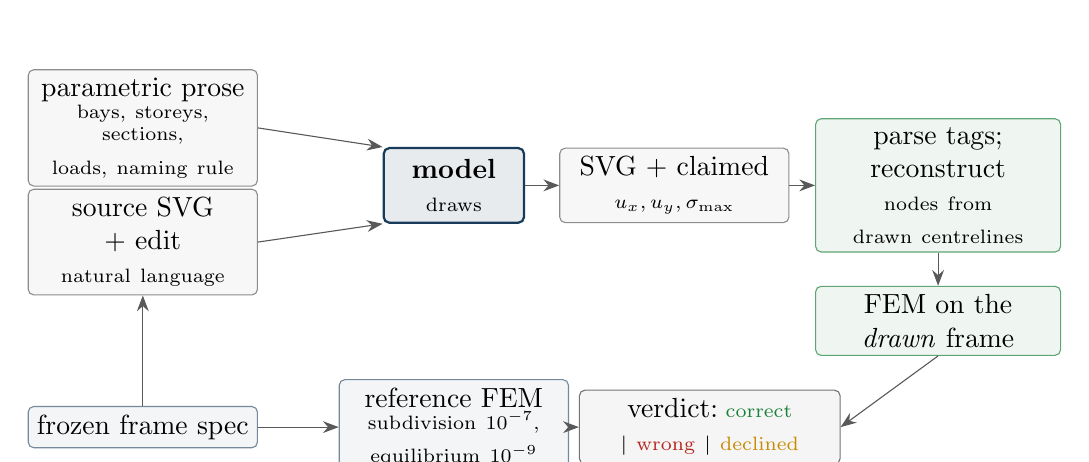
\begin{tikzpicture}[x=1cm,y=1cm,
  box/.style={draw=black!45,fill=black!3,rounded corners=2pt,align=center,inner sep=3pt,text width=27mm},
  model/.style={draw=researchblue,fill=researchblue!10,rounded corners=2pt,align=center,inner sep=4pt,thick,text width=15mm},
  check/.style={draw=okgreen!70,fill=okgreen!7,rounded corners=2pt,align=center,inner sep=3pt,text width=29mm},
  oracle/.style={draw=researchblue!60,fill=researchblue!5,rounded corners=2pt,align=center,inner sep=3pt,text width=27mm},
  verdict/.style={draw=black!55,fill=black!4,rounded corners=2pt,align=center,inner sep=3pt,text width=31mm},
  ar/.style={-{Stealth[length=2mm]},draw=black!65}]

\node[box]     (txt)   at (0,1.45)    {parametric prose\\\scriptsize bays, storeys, sections,\\\scriptsize loads, naming rule};
\node[box]     (edt)   at (0,0)       {source SVG $+$ edit\\\scriptsize natural language};
\node[model]   (m)     at (3.95,0.72) {\textbf{model}\\\scriptsize draws};
\node[box]     (out)   at (6.75,0.72) {SVG $+$ claimed\\\scriptsize $u_x,u_y,\sigma_{\max}$};
\node[check]   (parse) at (10.1,0.72) {parse tags; reconstruct\\\scriptsize nodes from drawn centrelines};
\node[check]   (refem) at (10.1,-1.0) {FEM on the \emph{drawn} frame};
\node[oracle]  (spec)  at (0,-2.35)   {frozen frame spec};
\node[oracle]  (ref)   at (3.95,-2.35){reference FEM\\\scriptsize subdivision $10^{-7}$,\\\scriptsize equilibrium $10^{-9}$};
\node[verdict] (v)     at (7.2,-2.35) {verdict:\;\scriptsize\textcolor{okgreen}{correct} $\mid$ \textcolor{badred}{wrong} $\mid$ \textcolor{warnamber}{declined}};

\draw[ar] (txt.east) -- (m.north west);
\draw[ar] (edt.east) -- (m.south west);
\draw[ar] (m) -- (out);
\draw[ar] (out) -- (parse);
\draw[ar] (parse) -- (refem);
\draw[ar] (spec) -- (ref);
\draw[ar] (spec.north) -- (edt.south);
\draw[ar] (ref.east) -- (v.west);
\draw[ar] (refem.south) -- (v.east);
\end{tikzpicture}
\caption{Both arms feed one verifier. The frozen specification builds the reference and the source
drawing, but never reaches the model; agreement is therefore evidence rather than construction. The
deterministic exporter that draws from the specification is the oracle --- its own drawings pass every
check by construction, which is the harness's positive control.}
\end{figure}

Two consequences follow. The exporter path means a correct drawing can always be produced from a solved
specification without a model at all, so the model is only ever being asked whether it can reach the same
place unaided. And because the checks run on reconstructed geometry, a drawing that merely copies its
input fails the edited-frame FEM outright --- which is the defence against the copy-reward trap that
makes similarity metrics useless on edit tasks.

\paragraph{Where Astra sits.} Astra appears in this brief only as the \emph{subject under test}. It is
run end-to-end against both arms with no tools, to establish what a frontier model reaches unaided and
therefore what the pipeline has to supply for itself. It is not a component of Figure~1, and nothing
here is designed around continued access to it.

% =====================================================================
\section{Dataset}

Everything is generated; no real-drawing corpus is involved. Frames are ordered by degree of static
indeterminacy, $i = 3m + r - 3j$ for $m$ members, $r$ reaction components and $j$ joints, because a
determinate frame yields to statics alone while an indeterminate one needs the simultaneous stiffness
system --- the part that must be carried out unaided.

\begin{center}
\begin{tabular}{llrll}
\toprule
Set & Path & Tasks & Input & Role \\
\midrule
text $\to$ SVG & \code{data/eng-svg-bench-text} & 24 & prose, 2.2--2.7\,kB & \textbf{benchmark} \\
SVG $\to$ SVG & \code{data/eng-svg-bench-edit} & 24 & drawing $+$ edit, 3.7--11.7\,kB & \textbf{benchmark} \\
\addlinespace
pilot & \code{data/cad-astra-pilot} & 6 & JSON model & source of case A \\
frames & \code{data/eng-frame-bench} & 18 & JSON model & source of case B \\
frames XL & \code{data/eng-frame-bench-xl} & 6 & JSON model & source of case B \\
\bottomrule
\end{tabular}
\end{center}

The two benchmark arms span 3 to 21 members and $i = 3$ to $27$. \textbf{Neither supplies a structured
model}, which is what separates them from the three lower sets: those handed the model over as JSON, and
the measured results in Sections~5 and~6 were all obtained under that easier condition. A record earned
with coordinates supplied does not transfer to a task where they must be derived, so the two arms need
measuring from scratch.

Each task carries the frozen physical model, the prompt, ground-truth member lengths, the FEM reference
(displacements, peak stress, per-member stresses, reactions, equilibrium residual), the deflection and
stress limits, the physical-to-SVG mapping, a model hash, and the exporter's own reference drawing. A
reference is admitted only after member-subdivision invariance at $10^{-7}$ and a dimensionally
normalised equilibrium residual below $10^{-9}$ --- the force and moment parts of that residual carry
different units and need separate scales, or a large frame is rejected for being large rather than wrong.
Nine checks pass on each arm, including that the exporter drawing scores as a pass and that FEM of its
reconstructed geometry matches the reference.

Each description ends with a checksum --- \emph{``derived correctly this frame has exactly 8 nodes and 8
members''} --- so a mis-derivation is detectable rather than silent. The prose is templated, so a
systematic failure warrants inspecting the description for ambiguity before it is attributed to the model.

\section{Failure case A: a correct drawing carrying a false claim}

The first case is the one the verification layer exists for: everything a reader can see is right, and
the conclusion is wrong.

The task was an \emph{edit}. The model received the original two-storey setback frame, its SVG, and an
instruction to move the middle column grid from $x=3400$ to $x=4100$\,mm, raise the upper floor from
$y=6200$ to $y=6800$\,mm, and change the vertical load at node H to $-61$\,kN --- then to recompute
every dimension and every derived quantity. It did all of that in a single call with no tools. The
geometry check passes at 1\,mm, every joint closes, all eight member lengths are correct, and the
visible SVG results agree with the returned JSON. By every structural and drafting criterion the
drawing is sound.

\begin{figure}[H]
\centering
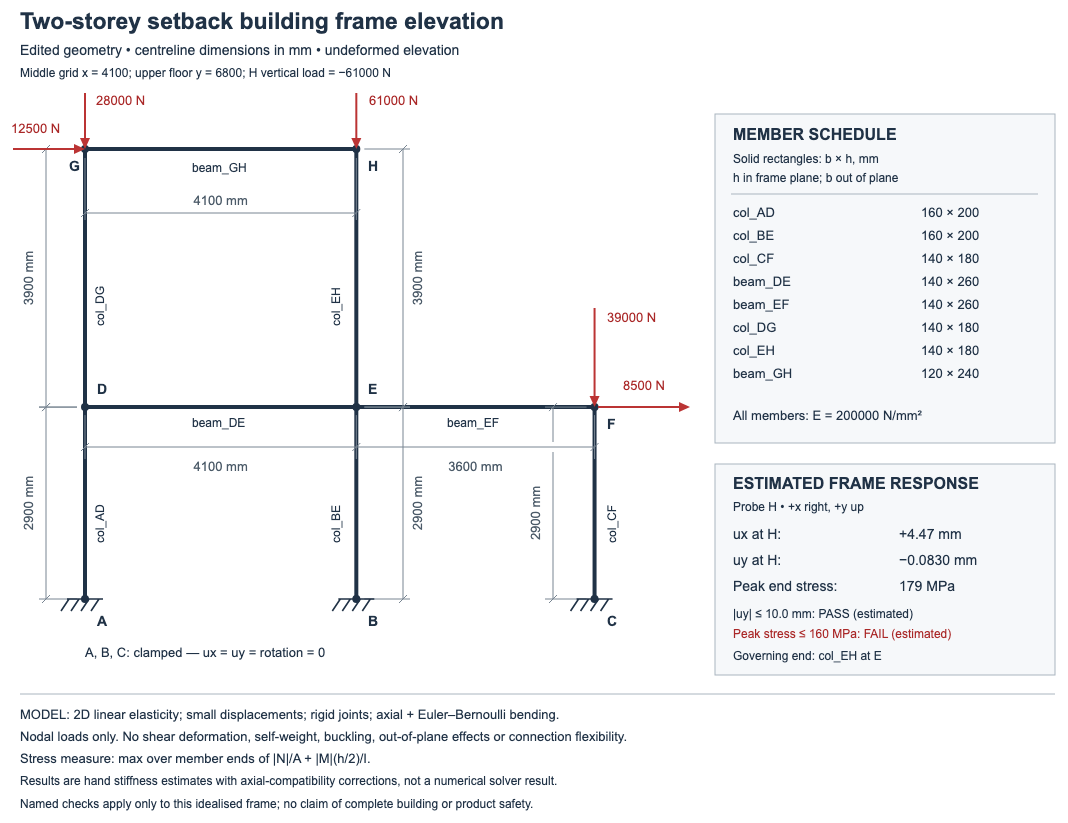
\includegraphics[width=0.87\textwidth]{../../paper/figures/fail_A_astra.png}
\caption{\code{building_edit}, 20 September pilot, unmodified output. The edit --- move the middle
grid to $x=4100$, raise the upper floor to $y=6800$, change the load at H to $-61$\,kN --- was applied
correctly. Geometry and all eight member dimensions pass at 1\,mm. The defect is confined to the
results panel.}
\label{fig:A}
\end{figure}

\begin{figure}[H]
\centering
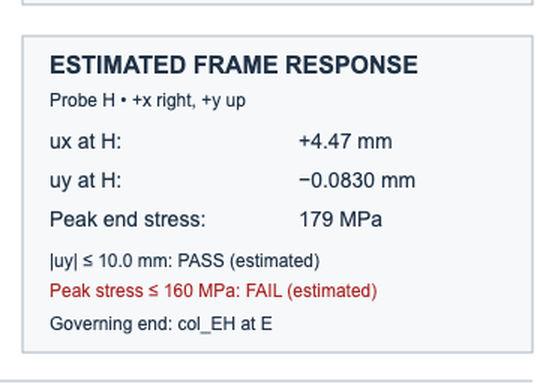
\includegraphics[width=0.50\textwidth]{../../paper/figures/fail_A_detail.png}
\caption{Detail of the same panel. Both displacements are right to 0.3\,\%. The peak stress is
\textbf{179\,MPa} against a reference of \textbf{20.356\,MPa}, a factor of 8.8 --- and the drawing
therefore declares the frame to \emph{fail} its 160\,MPa limit when its true peak is one eighth of it.}
\label{fig:Adetail}
\end{figure}

What makes this case instructive is how much the model got right on the way to the wrong number. It
named the governing location, \code{col_EH} at end E, which is genuinely the maximum. It stated the
correct extreme-fibre definition,
$\sigma_{\max} = \max\left(|N|/A + |M|(h/2)/I\right)$. It solved the displacements essentially exactly.
It also labelled the panel \emph{estimated} rather than claiming a solver run. Every diagnostic signal
was right; only the arithmetic that reaches the page was wrong.

The consequence is not academic. A drawing released in this state condemns a safe structure and
triggers a redesign, and no reader could detect the error from the drawing.

\textbf{It does not reproduce.} Three fresh samples at the identical protocol returned 20.4\,MPa. Under
the project's own admission rule --- three completed samples all failing --- this is not a systematic
capability limit. It is a sporadic error, observed once in 42 completed samples.

% =====================================================================
\section{Failure case B: a correct drawing that refuses to conclude}

The second case is the one that reproduces. As the frame grows, the model keeps drafting to the same
standard but stops short of the analysis rather than guessing at it.

\begin{figure}[H]
\centering
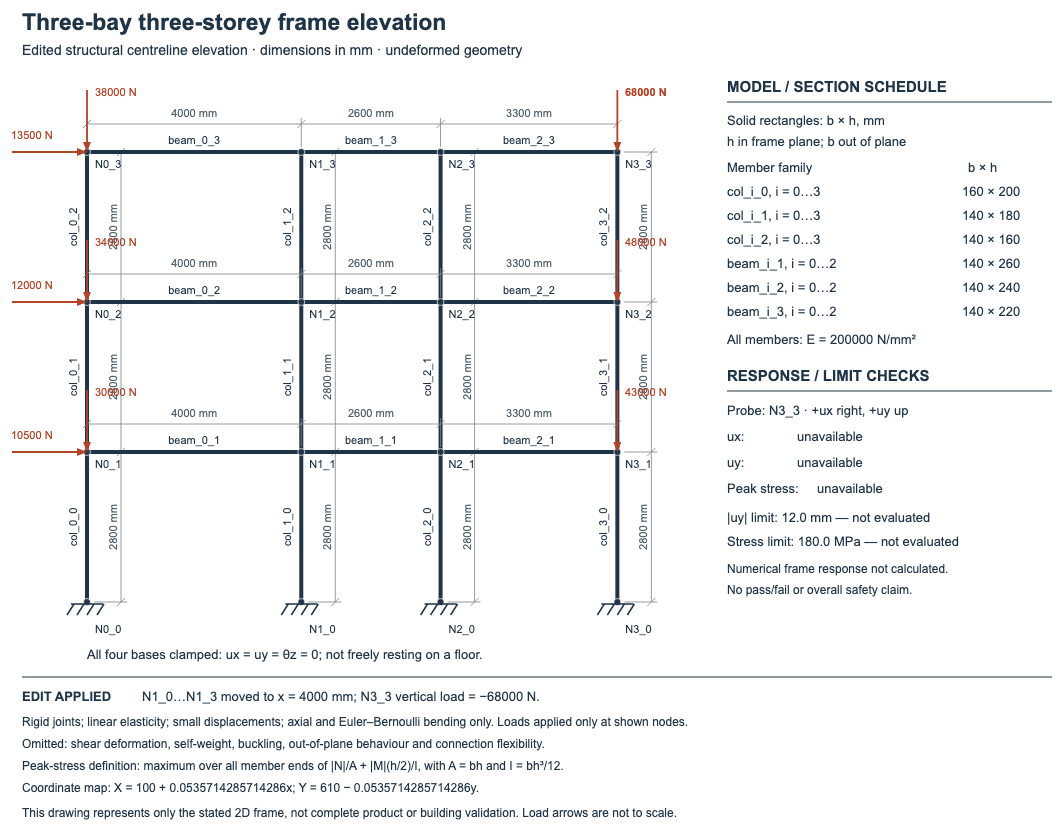
\includegraphics[width=0.87\textwidth]{../../paper/figures/fail_B_declined.png}
\caption{\code{threebay_three_edit}, 21 members, $i=27$, unmodified output. The frame, all 21 member
dimensions, the applied edit and the modelling notes are complete and correct. The response panel is
empty.}
\label{fig:B}
\end{figure}

\begin{figure}[H]
\centering
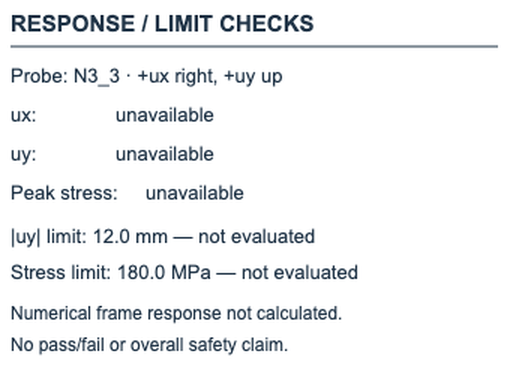
\includegraphics[width=0.46\textwidth]{../../paper/figures/fail_B_detail.png}
\caption{Detail. The model returns \code{status: "unavailable"}, declines both limit checks and states
\emph{``no pass/fail or overall safety claim''}. It gave a specific reason: the edited frame stiffness
solution and member-end force recovery were not performed.}
\label{fig:Bdetail}
\end{figure}

This is the behaviour that \emph{does} reproduce, and it is tied to frame size.

\begin{center}
\begin{tabular}{rrrrr}
\toprule
Members & Samples & \textcolor{okgreen}{Correct} & \textcolor{badred}{Wrong} & \textcolor{warnamber}{Declined} \\
\midrule
3--18 & 35 & 34 & 1 & 1 \quad(3\,\%) \\
20--21 & 7 & 3 & 0 & \textbf{4 \quad(57\,\%)} \\
\bottomrule
\end{tabular}
\end{center}

The contrast is significant at $p = 0.0015$ (two-sided Fisher exact); the 57\,\% rate carries a 95\,\%
Wilson interval of 25--84\,\%. Token budget is not the cause: declines finish cleanly after
6{,}600--8{,}100 completion tokens against a 32{,}000 cap, while successful answers on the same
instances use more. It is a boundary in willingness to attempt an unaided indeterminate solve, not in
drafting --- the drawing is always finished.

% =====================================================================
\section{What the two cases show together}

Accuracy does not decay with complexity; willingness does. In all 36 samples where a number was given
it was within tolerance, including at 21 members and $i = 27$, where the model returned 17.7\,MPa
against a reference of 17.6837. The model is either right or silent, with one observed exception.

That inverts the premise the programme was built on. The expectation was that the model would draw
plausibly and be numerically wrong, making verification a lie detector. Measured, the model is
numerically right whenever it commits and says so when it cannot. The verification layer's primary
value is therefore \textbf{completion} --- supplying the solve the model declines to attempt, so the
drawing is finished rather than rejected --- with silent-error detection as a secondary, still
necessary, guard that Figure~\ref{fig:Adetail} shows is not hypothetical.

\paragraph{What this says about the architecture.} The measurement lands exactly on the seam in
Figure~1. Geometry was never the problem: across all 42 samples the frames, dimensions and joints were
correct at every size, in both generation and editing. The failures were confined to the numbers ---
wrong once, refused five times. That is the empirical case for letting a model plan and edit while a
solver and a deterministic exporter own the quantities, rather than asking the model to compute and
draw them together. It also sets the priority: the exporter and verifier stages are not defensive
scaffolding around a weak drafter, they are the stages that carry the only part of the job that
actually breaks.

One further caution, from our own harness: three results were initially recorded as model failures for
omitting \code{mm} on individual dimension labels, when each drawing declared its units once in the
notes. Stating units once is standard drafting practice; the checker was penalising correct work. Two
of the four leads chased in this study were artefacts of measurement rather than of the model.

% =====================================================================
\section{Scope and reproduction}

Planar rigid-jointed frames, linear elastic, small displacement, nodal loads,
rectangular sections; self-weight, shear deformation, buckling and connection flexibility are outside
the model. Scoring audits tagged geometry and numbers, not rendering quality, layers or title-block
convention. All runs used \code{gpt-6-astra} at medium reasoning effort.

Two limits on the data itself. The boundary is bracketed rather than resolved: 18 members passed twice,
20 and 21 declined in 4 of 7 samples, and member count cannot be separated from degree of indeterminacy
because they rise together in this generator. And one instance, \code{twobay_four_generate} at 20
members, rests on its single screened sample --- its confirmation runs were cut off when API credits
were exhausted, and are recorded as excluded rather than counted as failures.

\paragraph{Reproducing.}
From \code{cvpr2027/} with \code{PYTHONPATH=src}:
\begin{verbatim}
../.venv/bin/python scripts/eng_frame_bench.py build
../.venv/bin/python scripts/eng_frame_bench.py verify
../.venv/bin/python scripts/cad_astra_benchmark.py run --data data/eng-frame-bench \
    --output runs/<fresh> --samples 3
../.venv/bin/python scripts/eng_frame_report.py
\end{verbatim}
Full study, statistics and limits: \code{reports/ENG_FRAME_FAILURE_BOUNDARY_20260922.md} and
\code{docs/latex/eng_frame_failure_study.tex}.

\end{document}
